\section{Brugervejledning}

Når du åbner appen vil du blive mødt med forsiden for den nuværende sæson. Her har du mulighed for at designe og planlægge din have. Som udgangspunkt, er haven delt op i to: udendørs køkkenhave og drivhus. Trykker du på en af kategorierne, vil som førstegangsbruger blive mødt med en tom have.

\subsection{Design din have}

\begin{minipage}{0.4\textwidth}
\begin{figure}[H]
    \centering
    \frame{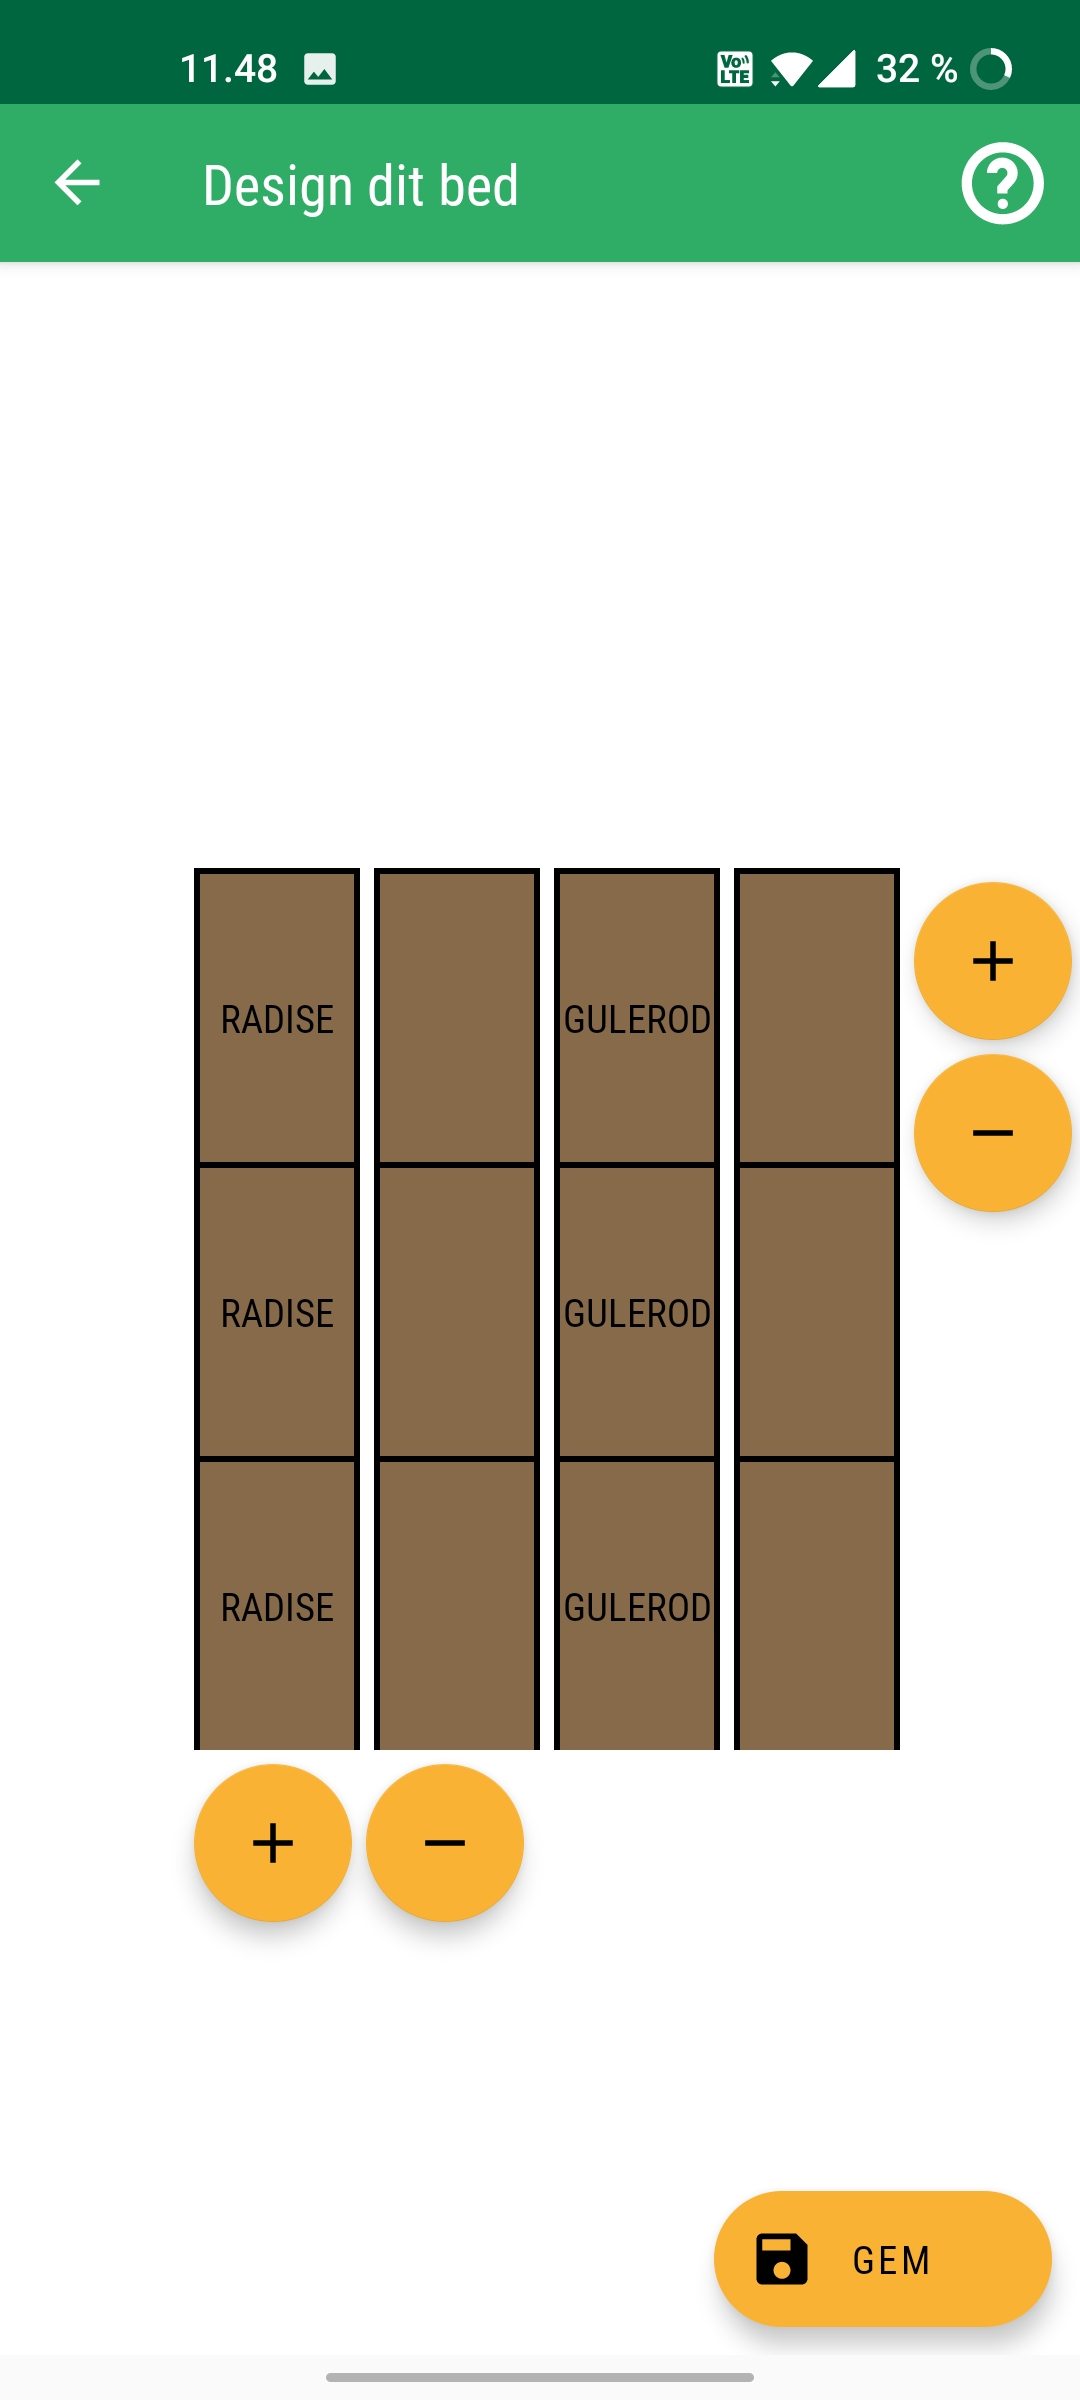
\includegraphics[width=\textwidth]{img/screenshot-nyt-bed.jpg}}
    \caption{Opret et nyt bed eller område}
\end{figure}
\end{minipage} \hfill
\begin{minipage}{0.55\textwidth}    
Når du har valgt 'Udendørs' eller 'Drivhus' kan du se og oprette bede, eller andre forskellige områder du ønsker at repræsentere i appen. Tryk på plus-knappen nede i hjørnet for at komme i gang.
Hvert felt i bedet kan indeholde en plante. Tryk på feltet for at få en liste over planter og vælg, hvilken du ønsker at placere. Du kan ændre bedets størrelse på plus- og minus-knapperne til højre og for neden. Hvis dit bed ikke er firkantet, anbefaler vi, at du laver bedet større end dit fysiske bed og blot udfylder de felter, der bedst repræsenterer en anden facon. Når du er færdig kan du klikke på gem og navngive dit bed. En måde, at navngive bede på, kan være at bruge typen af planter i bedet.
\end{minipage} 

\begin{minipage}{0.4\textwidth}
\begin{figure}[H]
    \centering
    \frame{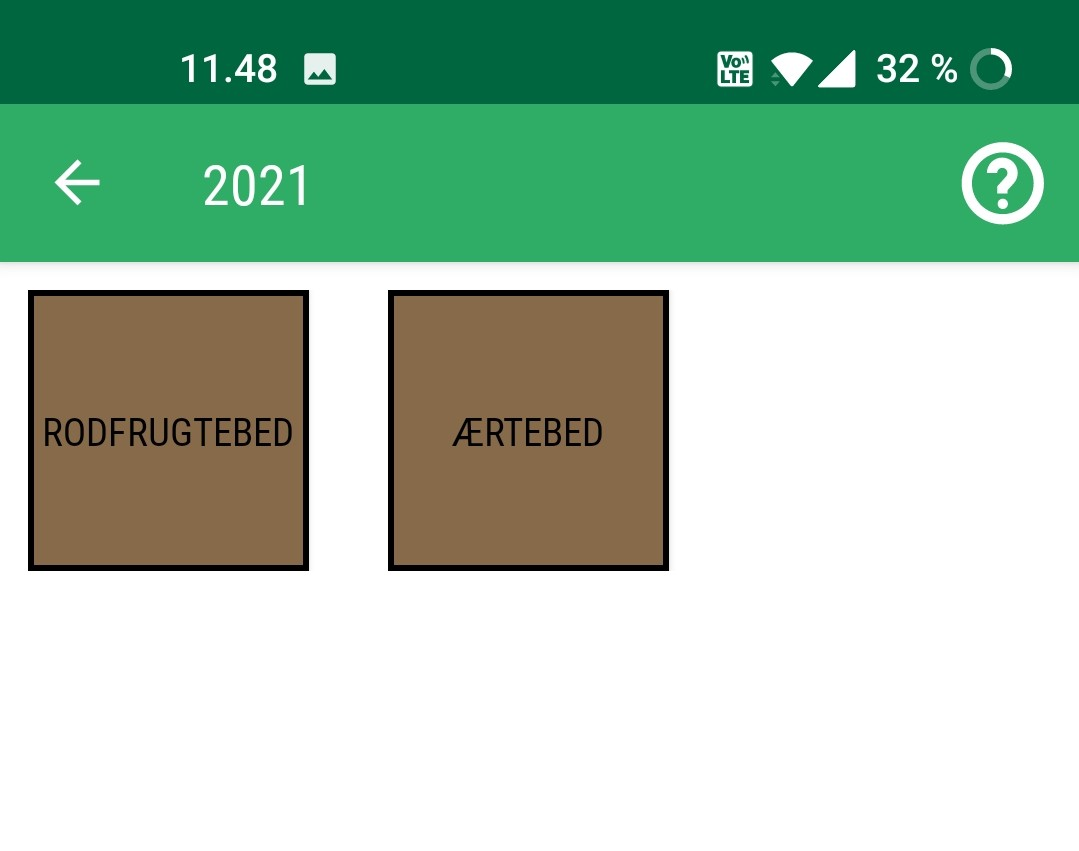
\includegraphics[width=\textwidth]{img/screenshot-oversigt-bede.jpg}}
    \caption{Oversigt over bede}
\end{figure}
\end{minipage} \hfill
\begin{minipage}{0.5\textwidth}
Når du har oprettet din have kan du se dem i den oversigt, der før var tom.
For at få det til at ligne din egen have mest muligt, kan du holde inde på et bed og trække i det for at skifte bedenes rækkefølge. Dette kan også hjælpe appen til at holde styr på sædskifte. Læs mere om dette under sædskifte.
\end{minipage}

\begin{minipage}{0.4\textwidth}
\begin{figure}[H]
    \centering
    \frame{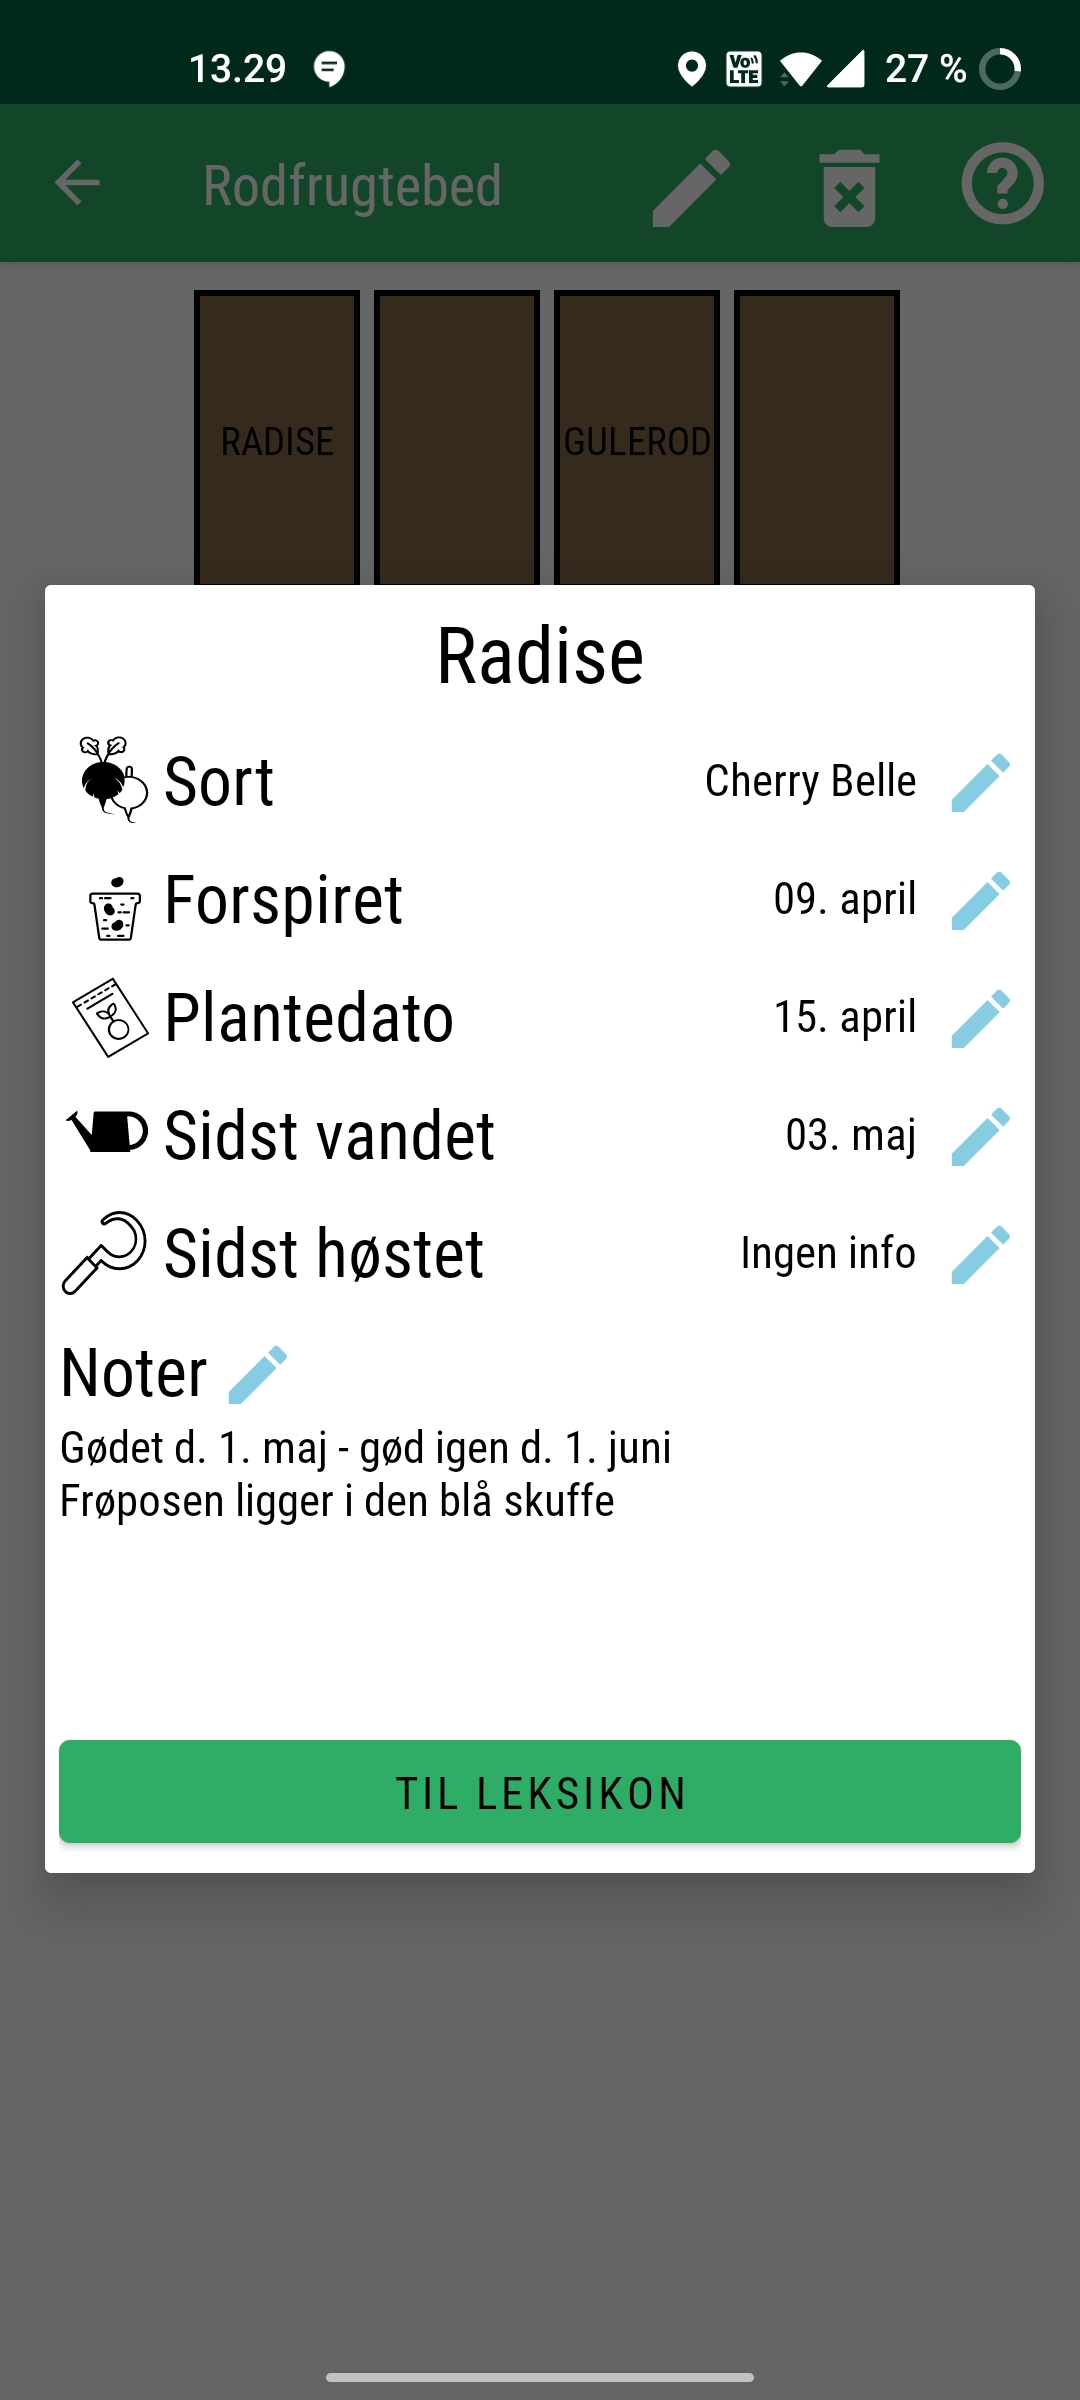
\includegraphics[width=\textwidth]{img/screenshot-plante-i-bed.jpg}}
    \caption{Tilpasning af detaljer om en plantet radise}
\end{figure}
\end{minipage} \hfill
\begin{minipage}{0.5\textwidth}
Hvis du trykker på et bed, har du mulighed for at redigere eller slette bedet øverst til højre. Når du redigerer bedet kan du ændre størrelsen, planterne og afslutningvis kan du ændre navnet, når du trykker på gem. Hvis du trykker på en bestemt plante i bedet, kan du indtaste detaljer, der vedrører denne plante specifikt. Her kan du f.eks. indtaste en bestemt sort, holde styr på hvornår den er blevet vandet og skrive noter. Hvis du vil have mere generel info om planten, kan du trykke på "Til leksikon".
\end{minipage}

\subsection{Planlæg kommende sæsoner og se historik}
\begin{minipage}{0.4\textwidth}
\begin{figure}[H]
    \centering
    \frame{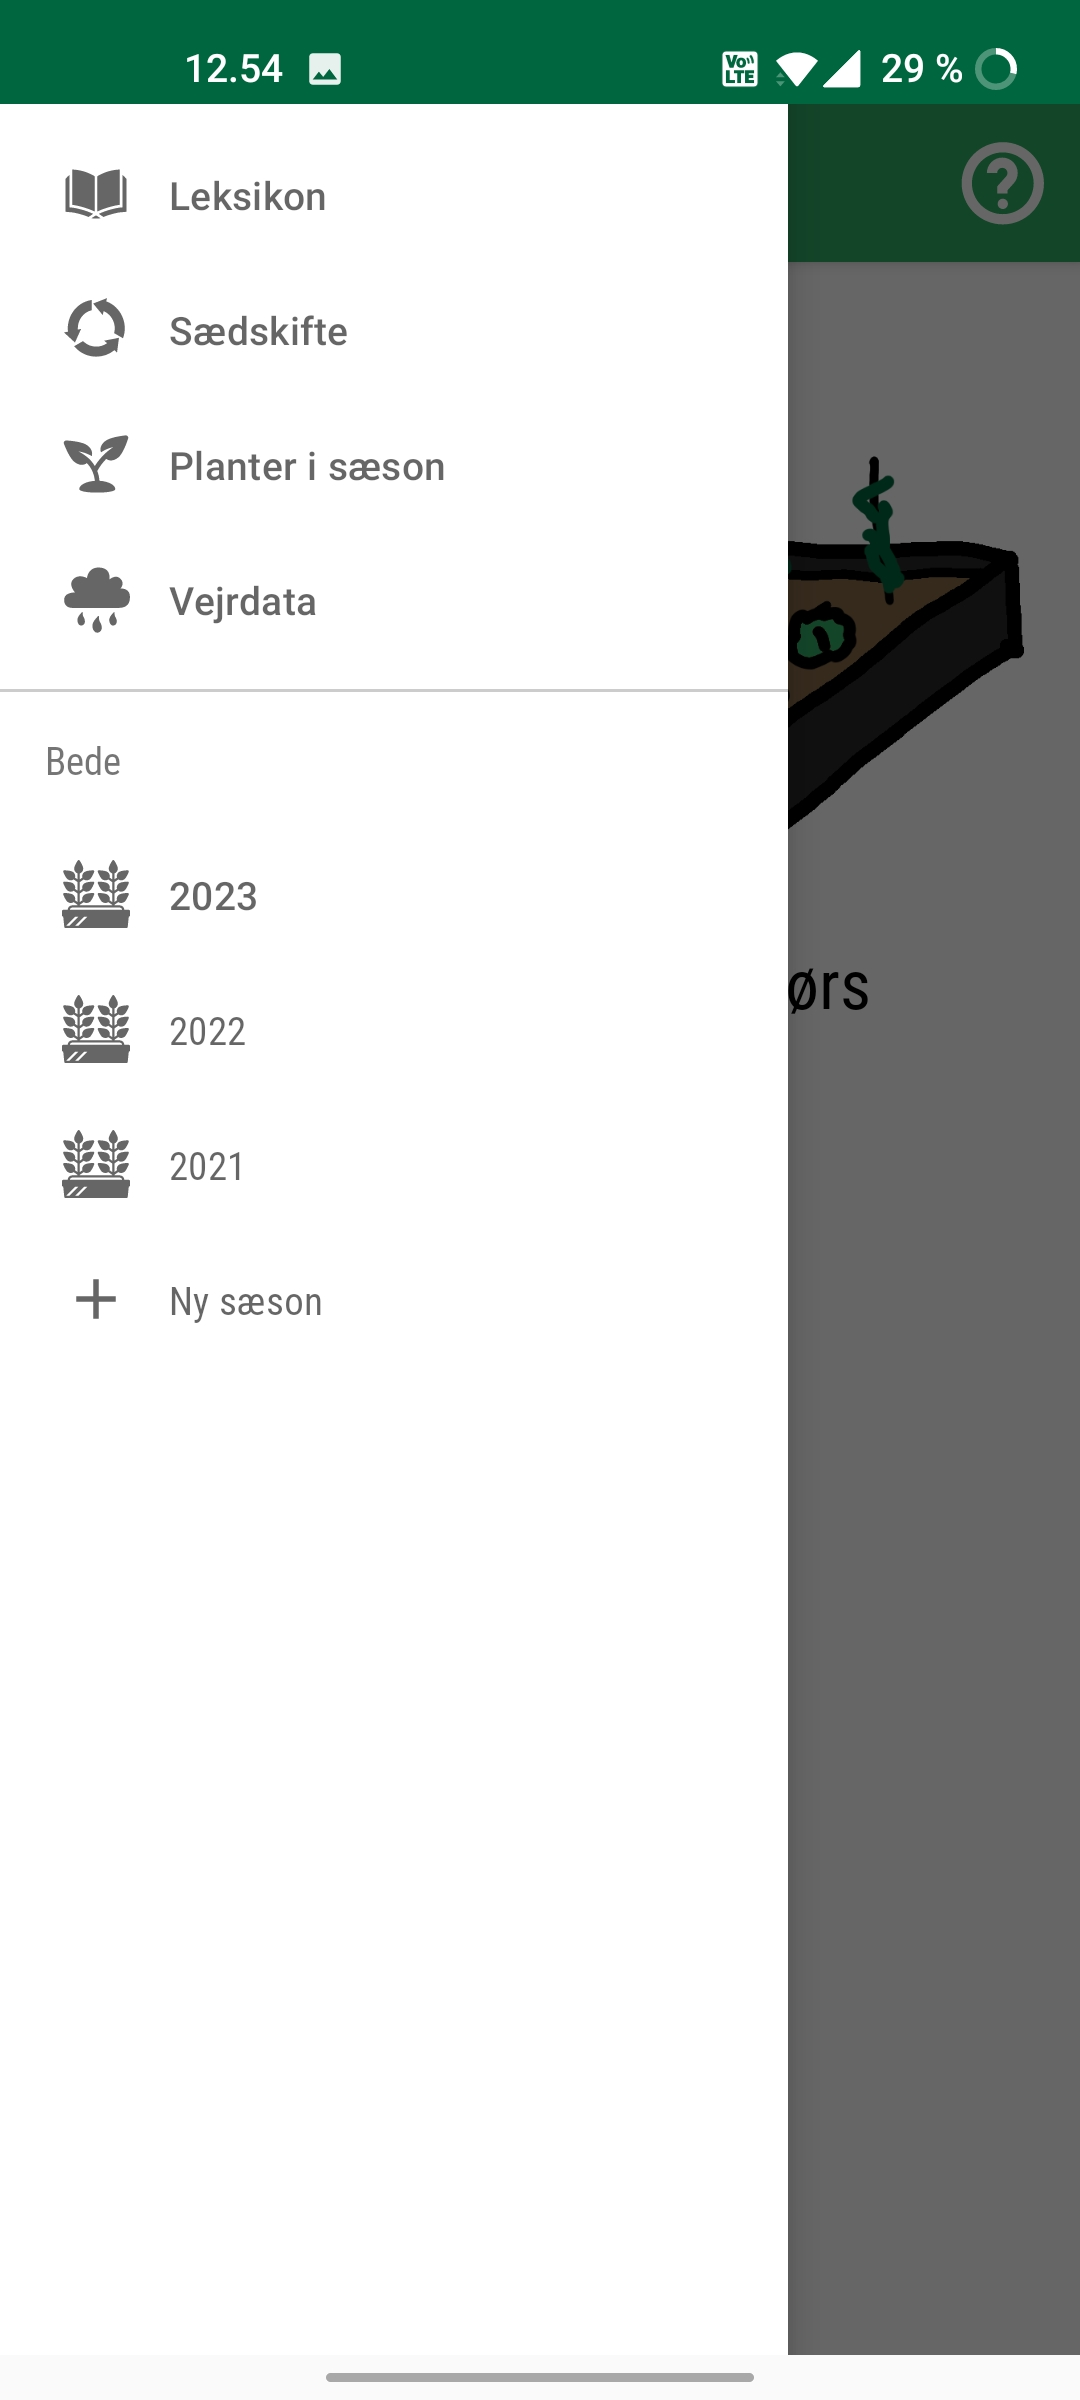
\includegraphics[width=\textwidth]{img/screenshot-sidemenu.jpg}}
    \caption{Side-menuen}
\end{figure}
\end{minipage} \hfill
\begin{minipage}{0.55\textwidth}
I side-menuen, som kan åbnes øverst til venstre, kan du se en oversigt over alle de oprettede sæsoner. Når du åbner appen første gang, vil der automatisk være oprettet en sæson for det nuværende årstal. Du kan oprette en ny sæson ved at trykke på "Ny sæson", og indtaste hvilket årstal, sæsonen skal repræsentere. Du kan bruge denne funktion til at planlægge i forvejen, og dermed f.eks. oprette næste sæson i god tid. Du kan også vælge at oprette de nye sæsoner efterhånden som du når dertil. De gamle sæsoner vil altid være gemt, og det vil derfor være nemt at trykke tilbage og se, hvordan din have så ud tidligere.
\end{minipage} 

\subsection{Se og opret planter}
Tryk på side-menuen og åbn leksikonnet. Her vil du få en oversigt over alle de planter, som appen per default har. Du kan søge efter en bestemt plante eller blot scrolle gennem listen. Hvis du trykker på en plante, vil du blive ført til en informationsside, hvor du kan se alt det data, som appen kender om den givne plante. Hvis du savner en plante, gerne vil have en seperat plante i appen for en bestemt sort eller lignende, kan du i bunden vælge "Ny plante". Her har du mulighed for at oprette dine egne planter og derefter bruge dem præcis som de prædefinerede.

\subsection{Få styr på sædskifte}

\subsection{Hvilke planter er i sæson?}

\subsection{Vurder vanding i forhold til lokalvejret}
